\chapter{Hadoop}
\label{cap:hadoop}

Uma das soluções mais conhecidas para análise de dados em larga escala é o projeto Apache Hadoop, concebido por Doug Cutting\footnote{\url{http://en.wikipedia.org/wiki/Doug_Cutting}}, o mesmo criador da biblioteca de busca textual Apache Lucene\footnote{\url{http://lucene.apache.org/core/}} \cite{white2012}. Os componentes principais desta ferramenta consistem em um sistema de arquivos distribuídos para ser executado em \textit{clusters}\footnote{Um \textit{cluster} pode ser classificado como um aglomerado de computadores que simulam o comportamento de uma única máquina. Segundo \citeonline{tanenbaum2003}, são CPUs fortemente acopladas que não compartilham memória.} compostos por máquinas de baixo custo, e também pelo \textit{framework} de programação paralela MapReduce. Ambos foram inspirados nos trabalhos publicados por \citeonline{ghemawatGfs2003} e \citeonline{ghemawatMapreduce2008}, e são objetos de estudo deste capítulo. O manual de instalação pode ser encontrado no apêndice \ref{apd-hadoop}.

\section{Hadoop Distributed File System}

Quando uma base de dados atinge a capacidade máxima de espaço provida por uma única máquina física, torna-se necessário distribuir esta responsabilidade com um determinado número de computadores. Sistemas que gerenciam o armazenamento de arquivos em uma ou mais máquinas interligadas em rede são denominados sistemas de arquivos distribuídos \cite{white2012}. 

Para \citeonline{coulouris2007}, um sistema de arquivos distribuído permite aos programas armazenarem e acessarem arquivos remotos exatamente como se fossem locais, possibilitando que os usuários acessem arquivos a partir de qualquer computador em uma rede. Questões como desempenho e segurança no acesso aos arquivos armazenados remotamente devem ser comparáveis aos arquivos registrados em discos locais.

De acordo com \citeonline{white2012} seu funcionamento depende dos protocolos de rede que serão utilizados. Portanto todos os problemas relacionados a própria rede tornam-se inerentes a este tipo de abordagem, adicionando uma complexidade muito maior aos sistemas de arquivos distribuídos, por exemplo, em relação aos sistemas de arquivos convencionais.

No contexto Big Data, que engloba um volume muito grande de dados, a utilização de um mecanismo para armazenar informações ao longo de várias máquinas é indispensável. Neste sentido a camada mais baixa do Hadoop é composta por um sistema de arquivos distribuídos chamado Hadoop Distributed File System, ou HDFS.

O HDFS foi projetado para executar MapReduce \textit{jobs}\footnote{Um \textit{job} pode ser interpretado como uma unidade de trabalho a ser executada pelo sistema, ou seja, o próprio programa MapReduce.} que, por sua vez, realizam leitura, processamento e escrita de arquivos extremamente grandes \cite{venner2009}. Apesar de apresentar semelhanças com os sistemas de arquivos distribuídos existentes seu grande diferencial está na alta capacidade de tolerância a falhas, no baixo custo de hardware que é requerido e também na escalabilidade linear.

\subsection{Características Principais}

O HDFS foi projetado para armazenar arquivos muito grandes a uma taxa de transmissão de dados constante, sendo executado em \textit{clusters} com hardware de baixo custo \cite{white2012}. Suas principais características de \textit{design} podem ser descritas a seguir:

\begin{enumerate}

\item \textbf{Arquivos muito grandes:} Este sistema de arquivos distribuídos é capaz de armazenar arquivos que chegam a ocupar terabytes de espaço, portanto é utilizado por aplicações que necessitam de uma base de dados extremamente volumosa. Segundo \citeonline{shvachko2010}, os \textit{clusters} do Hadoop utilizados pela Yahoo\footnote{\url{http://pt.wikipedia.org/wiki/Yahoo!}} chegam a armazenar 25 petabytes de dados.

\item \textit{\textbf{Streaming data access:}} Operações de leitura podem ser realizadas nos arquivos quantas vezes forem necessárias, porém um arquivo pode ser escrito apenas uma única vez. Esta abordagem pode ser descrita como \textit{write-once}, \textit{read-many-times} \cite{white2012}. Este sistema de arquivos distribuídos foi construído partindo da ideia que este modelo é o mais eficiente para processar os dados. O HDFS também realiza a leitura de qualquer arquivo a uma taxa constante, ou seja, a prioridade é garantir vazão na leitura e não minimizar a latência ou prover interatividade com aplicações em tempo real, como é realizado em sistemas de arquivos com propósito geral.

\item \textbf{Hardware de baixo custo:} O HDFS foi projetado para ser executado em hardwares que não precisam ter necessariamente alta capacidade computacional e também alta confiabilidade. O sistema foi desenvolvido partindo do pressuposto que a chance dos nós ao longo do \textit{cluster} falharem é extremamente alta, portanto mecanismos de tolerância a falha foram desenvolvidos para contornar este problema, permitindo uma maior flexibilidade quanto ao uso de diferentes tipos de hardwares. A tabela \ref{tab-hardware} apresenta as configurações das máquinas utilizadas pelo \textit{cluster} Hadoop presente na empresa Yahoo.

\end{enumerate}

\begin{table}[!ht]
\begin{center}
  \begin{tabular}{|p{3cm}|p{2cm}|p{3cm}|p{4cm}|}
	\hline
	Processador (CPU) & Memória RAM  & Espaço em disco & Sistema Operacional
	\\ \hline
	2 quad-core de 2 a 2,5 GHz & 16 a 24 GB & 4 discos SATA de 1 Terabyte & Red Hat Enterprise Linux Server
	\\ \hline
  \end{tabular}
  \captionsetup{justification=centering}
  \caption[Configurações do cluster Yahoo]{Configurações do cluster Yahoo
  \protect\linebreak Fonte: Adaptado de \cite{white2012} e \cite{shvachko2010}}
\label{tab-hardware}
\end{center}
\end{table}
\FloatBarrier

\subsection{Divisão em Blocos}

Um disco é dividido em vários blocos com tamanho fixo, os quais compõe a menor estrutura de dados, onde são realizadas escritas e leituras. Em sistemas de arquivos convencionais cada bloco não ocupa mais que alguns KB de espaço, geralmente 512 bytes, esta informação é totalmente transparente para o usuário do sistema \cite{white2012}. Ele deve apenas realizar operações sobre arquivos de diferentes tamanhos.

O HDFS também possui o conceito de blocos, porém estes possuem tamanho bem maior, por padrão ocupam 64MB de espaço. Cada arquivo criado no sistema é quebrado em blocos com estas características, no qual cada um é salvo como uma unidade independente, podendo estar localizado em qualquer nó do \textit{cluster}. O HDFS foi projetado para armazenar arquivos que ocupam grande quantidade de espaço em disco, portanto com blocos de tamanho elevado o tempo de busca no disco é reduzido significativamente.

A figura \ref{fig-hdfs-blocos} ilustra como ocorre o armazenamento no \textit{cluster} HDFS. Quando um arquivo é escrito no sistema é realizada sua divisão em blocos, em seguida eles são espalhados pelos \textit{datanodes}, os quais são responsáveis por armazenar fisicamente estes blocos. A máquina central \textit{namenode} possui apenas o registro da localização exata de cada bloco no \textit{cluster}. Os conceitos sobre \textit{namenode} e \textit{datanode} são apresentados na seção \ref{sec-hdfs-arquitetura}.

\begin{figure}[ht!]
	\centering
	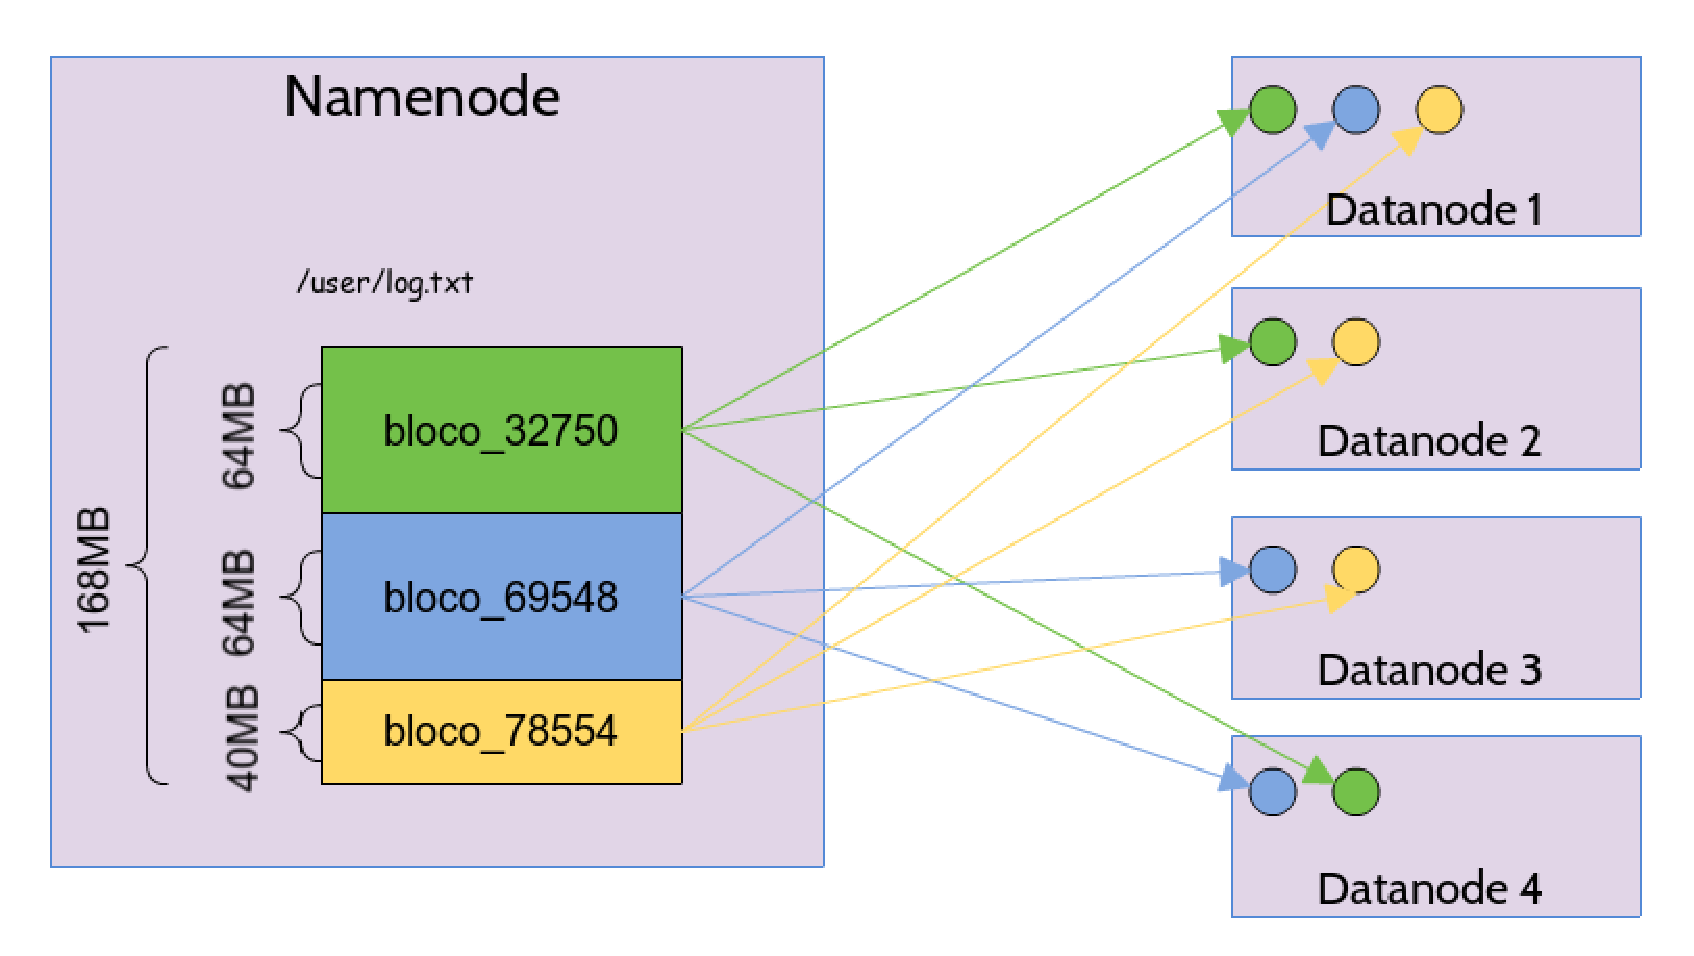
\includegraphics[keepaspectratio=true,scale=0.5]
	  {figuras/hdfs-blocos.eps}
	\caption[Divisão de Arquivos em Blocos no HDFS]{Divisão de Arquivos em Blocos no HDFS
	\protect\linebreak Fonte: Autor}
	\label{fig-hdfs-blocos}
\end{figure}
\FloatBarrier

A utilização de blocos permite simplificar o processo de gerenciamento do armazenamento dos dados. Uma vez que possuem tamanho fixo a tarefa de calcular a quantidade de blocos necessária para todo disco torna-se uma tarefa mais simples. Segundo \citeonline{white2012}, esta abordagem também permite que blocos sejam replicados pelo sistema de arquivos, provendo tolerância a falhas e uma maior disponibilidade dos dados. No exemplo abordado pela figura \ref{fig-hdfs-blocos} é possível perceber que o fator de replicação aplicado ao HDFS possui valor três. Desta forma cada bloco é copiado para três máquinas diferentes ao longo do \textit{cluster}.

\subsection{Arquitetura}
\label{sec-hdfs-arquitetura}

Para compreender a arquitetura do HDFS é necessário uma introdução ao GFS, o sistema de arquivos distribuídos proposto pela Google\footnote{http://pt.wikipedia.org/wiki/Google}, no qual foi projetado para atender a alta e crescente demanda de processamento de dados em larga escada encontrada na empresa. O GFS possui os mesmos objetivos de um sistema de arquivos distribuídos convencional: performance, escalabilidade, confiabilidade e disponibilidade \cite{ghemawatGfs2003}. Porém as soluções dos sistemas existentes foram revistas e muitas questões de \textit{design} foram alteradas radicalmente. Desta forma foi possível garantir escalabilidade linear, utilização de hardwares de baixo custo e também escrita e leitura de arquivos na ordem de multi gigabytes através do padrão \textit{write-once}, \textit{read-many-times}. 

Um \textit{cluster} GFS é composto por um único \textit{master} e múltiplos \textit{chunkservers}, os quais são acessados por múltiplos clientes \cite{ghemawatGfs2003}. Esta abordagem é baseada no tipo de arquitetura mestre/escravo. Ambos são executados como aplicações em nível de usuário em máquinas com sistema operacional GNU/Linux. A figura \ref{fig-gfs} ilustra a arquitetura do GFS para operações de leitura.

Neste modelo as aplicações que desejam utilizar o sistema de arquivos interagem primeiramente com o \textit{master}, responsável por armazenar o \textit{namespace} do GFS e também a localização dos blocos de arquivos ao longo do \textit{cluster}. É retornado para o cliente uma lista de \textit{chunkservers} que contém o arquivo solicitado. Posteriormente a aplicação acessa diretamente os \textit{chunkservers} para obter os blocos de arquivos.

\begin{figure}[ht!]
	\centering
	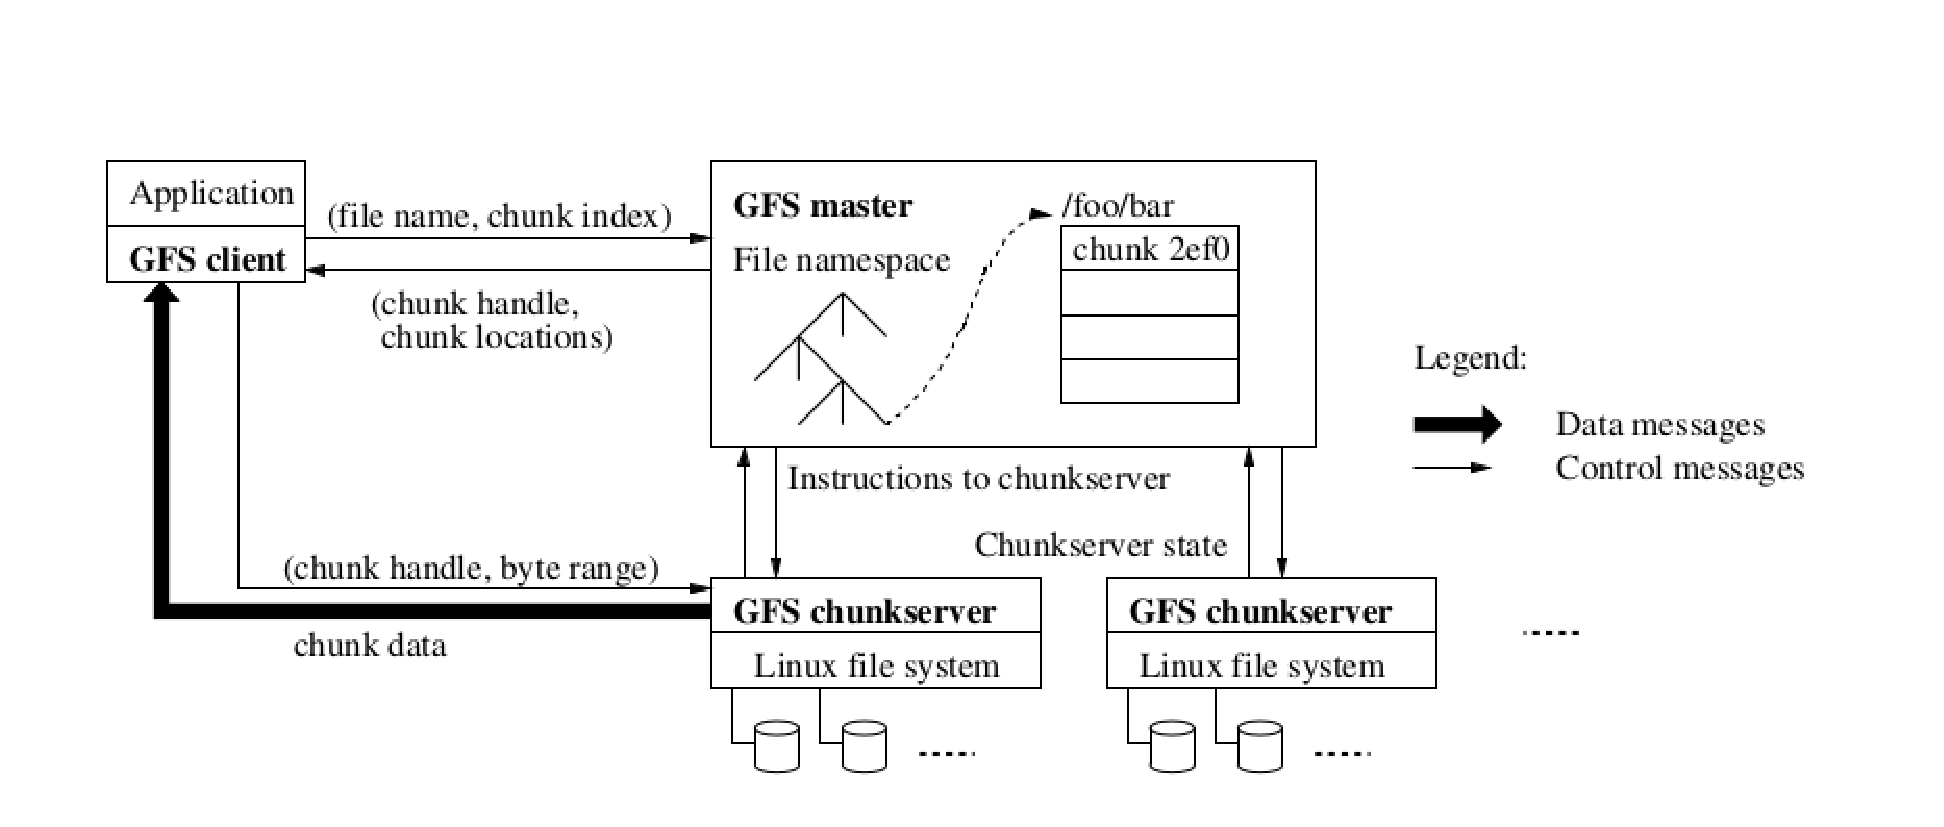
\includegraphics[keepaspectratio=true,scale=0.5]
	  {figuras/gfs.eps}
	\caption[Arquitetura do GFS]{Arquitetura do GFS
	\protect\linebreak Fonte: \cite{ghemawatGfs2003}.}
	\label{fig-gfs}
\end{figure}
\FloatBarrier

O HDFS foi construído a partir da arquitura apresentada por \citeonline{ghemawatGfs2003} para desenvolver o GFS. Todas as características abordadas nas seções anteriores, referentes ao HDFS, foram definidas com base neste trabalho. O HDFS apresenta uma alternativa \textit{open-source}\footnote{\textit{Open-source} são projetos de software que seguem o padrão para código aberto determindo pela OSI.} implementada em Java para o GFS.

Na solução apresentada pelo HDFS o nó mestre é identificado como \textit{namenode}. Seu papel consiste em gerenciar o \textit{namespace} do sistema de arquivos e também em controlar as requisições de clientes para acesso aos arquivos armazenados. Este componente mantém a árvore de diretórios e todos os metadados relacionados. Como descrito anteriormente, o HDFS quebra um arquivo em vários blocos e os espalha pelos diversos \textit{datanodes} do \textit{cluster}, o \textit{namenode} possui a tarefa de manter a localização de cada um destes blocos. Todas estas informações são armazenadas no disco local do servidor em dois arquivos: a imagem do sistema de arquivos e o registro de log \cite{white2012}. A imagem do sistema também é mantida em memória enquanto o \textit{cluster} está ativo, sendo constantemente atualizada.

Os \textit{datanodes} representam os nós escravos do HDFS. Eles são responsáveis por armazenar fisicamente os blocos de arquivos e recuperá-los quando solicitado. Estes blocos são escritos no sistema de arquivos da própria máquina onde o \textit{datanode} está localizado. Cada \textit{datanode} se comunica com o \textit{namenode} do \textit{cluster} através da camada de transporte TCP/IP, na qual é utilizada uma abstração do protocolo RPC \cite{hadoopSiteHDFS}. Periodicamente os \textit{datanodes} informam ao \textit{namenode} quais blocos cada um deles está armazenando, desta forma o \textit{namenode} gerencia todos os \textit{datanodes} presentes na rede. A figura \ref{fig-hdfs-arquitetura} ilustra a arquitetura do HDFS.

\begin{figure}[ht!]
	\centering
	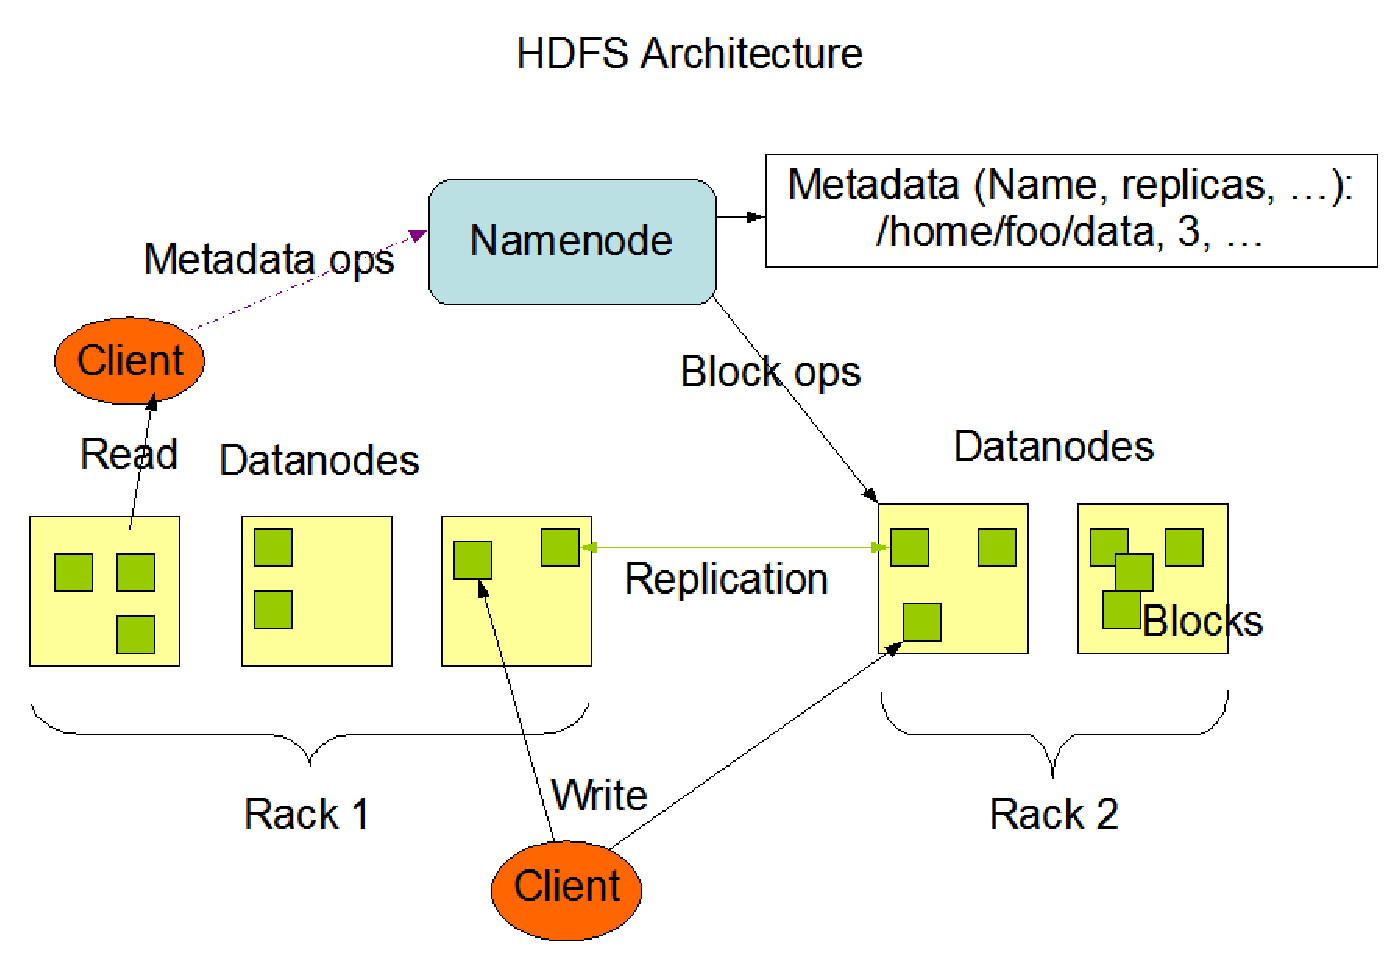
\includegraphics[keepaspectratio=true,scale=0.5]
	  {figuras/hdfs-arquitetura.eps}
	\caption[Arquitetura do HDFS]{Arquitetura do HDFS
	\protect\linebreak Fonte: \cite{hadoopSiteHDFS}}
	\label{fig-hdfs-arquitetura}
\end{figure}
\FloatBarrier

Na figura \ref{fig-hdfs-arquitetura} é possível perceber a semelhança do HDFS com a arquitetura do GFS. A ilustração apresenta um \textit{namenode} de um \textit{cluster} Hadoop, que mantém o \textit{namespace} do sistema de arquivos e recebe solicitações de aplicações clientes para escrita e leitura de arquivos. Posteriormente estas aplicações acessam os \textit{datanodes} diretamente para realizar estas operações sobre os blocos de arquivos, que estão persistidos e replicados ao longo do \textit{cluster}.

Assim como o GFS, o HDFS foi projetado para ser executado em distribuições GNU/Linux,  portanto para que uma máquina seja um namenode ou datanode é necessário apenas que possua uma JVM disponível juntamente com o sistema operacional adequado \cite{hadoopSiteHDFS}.

\subsection{Leitura e escrita}

As aplicações de usuários acessam o sistema de arquivos utilizando o HDFS \textit{Client}, uma biblioteca que disponibiliza uma interface de acesso aos arquivos do HDFS \cite{shvachko2010}. Assim como em sistemas de arquivos convencionais são permitidas operações de leitura, escrita e remoção de arquivos e diretórios. Segundo \citeonline{white2012}, o HDFS também utiliza uma interface POSIX para sistemas de arquivos, portanto as funções exercidas pelo \textit{namenode} e \textit{datanodes} tornam-se transparentes para o usuário final, pois apenas utiliza-se o \textit{namespace} do HDFS.

Para realizar operações de escrita o cliente deverá solicitar ao namenode a criação do arquivo desejado. Segundo \citeonline{white2012}, uma série de testes são realizadas para garantir que o cliente possui a permissão necessária e também para checar se o arquivo já existe no sistema. Caso esta etapa seja concluída com êxito o namenode retorna uma lista com o endereço de N datanodes disponíveis para receber o primeiro bloco do arquivo, onde N é o fator de replicação do HDFS, ou seja, o número de cópias que um bloco possui ao longo dos datanodes do \textit{cluster}.

O cliente realiza a escrita nos \textit{datanodes} através de um \textit{pipeline}. O bloco é copiado para o primeiro \textit{datanode} e em seguida repassado para o próximo, assim sucessivamente até os dados serem armazenados no último \textit{datanode} do \textit{pipeline}. A figura \ref{fig-hdfs-escrita} apresenta o fluxo do processo de escrita no HDFS.

\begin{figure}[ht!]
	\centering
	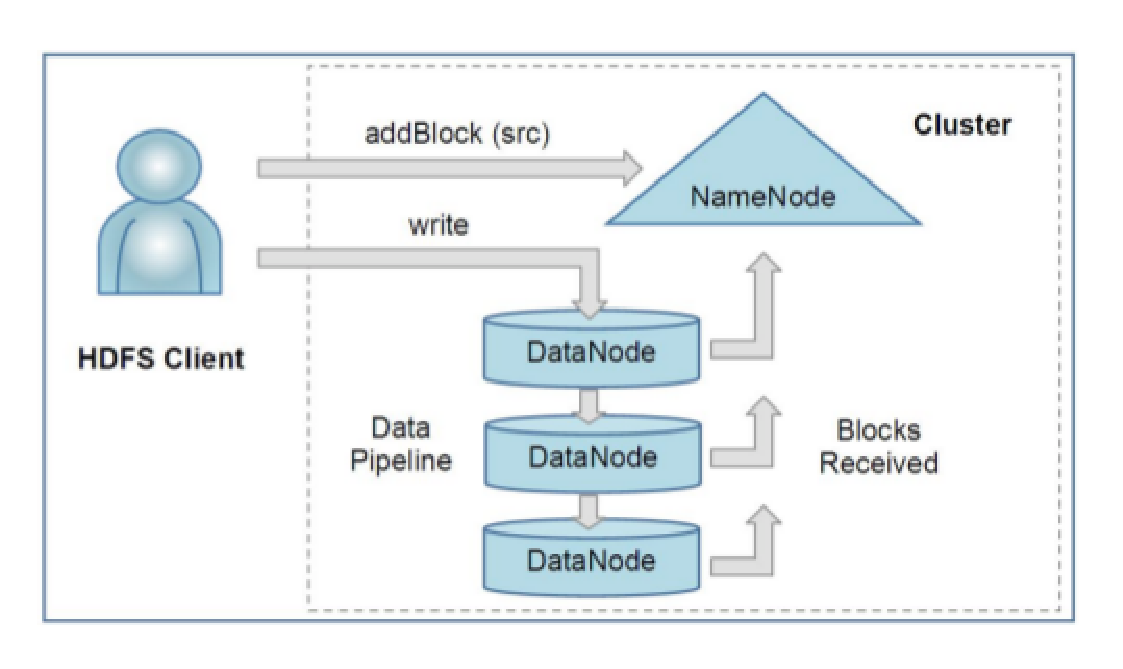
\includegraphics[keepaspectratio=true,scale=0.5]
	  {figuras/hdfs-escrita.eps}
	\caption[Operação de escrita no HDFS]{Operação de escrita no HDFS
	\protect\linebreak Fonte: \cite{shvachko2010}}
	\label{fig-hdfs-escrita}
\end{figure}
\FloatBarrier

Para cada bloco do arquivo é realizado este processo de \textit{pipeline}. Na figura \ref{fig-hdfs-escrita} é possível perceber que o fator de replicação do exemplo apresentado é igual a três, ou seja, cada bloco será repassado para três \textit{datanodes} diferentes. De acordo com \citeonline{shvachko2010}, para realizar o processo de leitura o cliente solicita ao \textit{namenode} a localização dos blocos que compõe o arquivo desejado, em seguida contacta diretamente os respectivos \textit{datanodes} para recuperar estes dados.

\section{MapReduce}

MapReduce pode ser definido como um paradigma de programação voltado para processamento em \textit{batch\footnote{Processamento em \textit{batch} (lotes) ocorre quando as entradas são lidas para posterior precessamento sequencial, sem interação com o usuário.}} de grande volume de dados ao longo de várias máquinas, obtendo resultados em tempo razoável \cite{white2012}. Utiliza-se o conceito de programação distribuída para resolver problemas, adotando a estratégia de dividi-los em problemas menores e independentes.

De acordo com \citeonline{ghemawatMapreduce2008}, o usuário deste modelo especifica uma função \textit{map}, que deverá processar um par \textit{\{chave, valor\}} gerando como produto conjuntos  intermediários de pares \textit{\{chave, valor\}}, e também define uma função \textit{reduce}, responsável por unir todos os valores intermediários associados a uma mesma chave.

Este modelo é baseado nas primitivas \textit{map} e \textit{reduce} presentes na linguagem \textit{Lisp} e também em muitas outras linguagens de programação funcional. Este paradigma foi adotado pois percebeu-se que vários problemas consistiam em realizar o agrupamento das entradas de acordo com uma chave identificadora, para então processar cada um destes conjuntos \cite{ghemawatMapreduce2008}.

Um programa MapReduce separa arquivos de entrada em diversas partes independentes que servem de entrada para as funções \textit{map}. As saídas destas funções são ordenadas por \textit{\{chave, valor\}} e posteriormente transformadas em entradas do tipo \textit{\{chave, lista(valores)\}} para a função \textit{reduce}, onde o resultado final será salvo em um arquivo de saída. A código \ref{cod-mapreduce-io} apresenta de maneira genérica as entradas e saídas das funções \textit{map} e \textit{reduce}.

\begin{lstlisting}[style=abnt,frame=single, 
		caption={[Entradas e saídas - MapReduce]Entradas e saídas - MapReduce
		\protect\linebreak Fonte: \cite{ghemawatMapreduce2008}},
		label=cod-mapreduce-io]
map     (k1,v1)         -> list(k2,v2)
reduce  (k2,list(v2))   -> list(v2)
\end{lstlisting}
\FloatBarrier

A grande contribuição desta abordagem está em disponibilizar uma interface simples e poderosa que permite paralelizar e distribuir computação em larga escala de forma automática \cite{ghemawatMapreduce2008}. O desenvolvedor precisa apenas se preocupar com as funções \textit{map} e \textit{reduce}, todo esforço para dividir o trabalho computacional ao longo das máquinas, entre outras questões operacionais, são de responsabilidade do próprio \textit{framework}.

A figura \ref{fig-mapreduce} ilustra um fluxo simplificado da execução de um programa MapReduce. As entradas são divididas em partes iguais denominadas \textit{input splits}, cada uma destas partes dão origem a uma \textit{map task}, responsável por gerar pares intermediários \textit{\{chave, valor\}}. Cada \textit{map task} realizada uma chamada a função \textit{map} definida pelo usuário.

\begin{figure}[ht!]
	\centering
	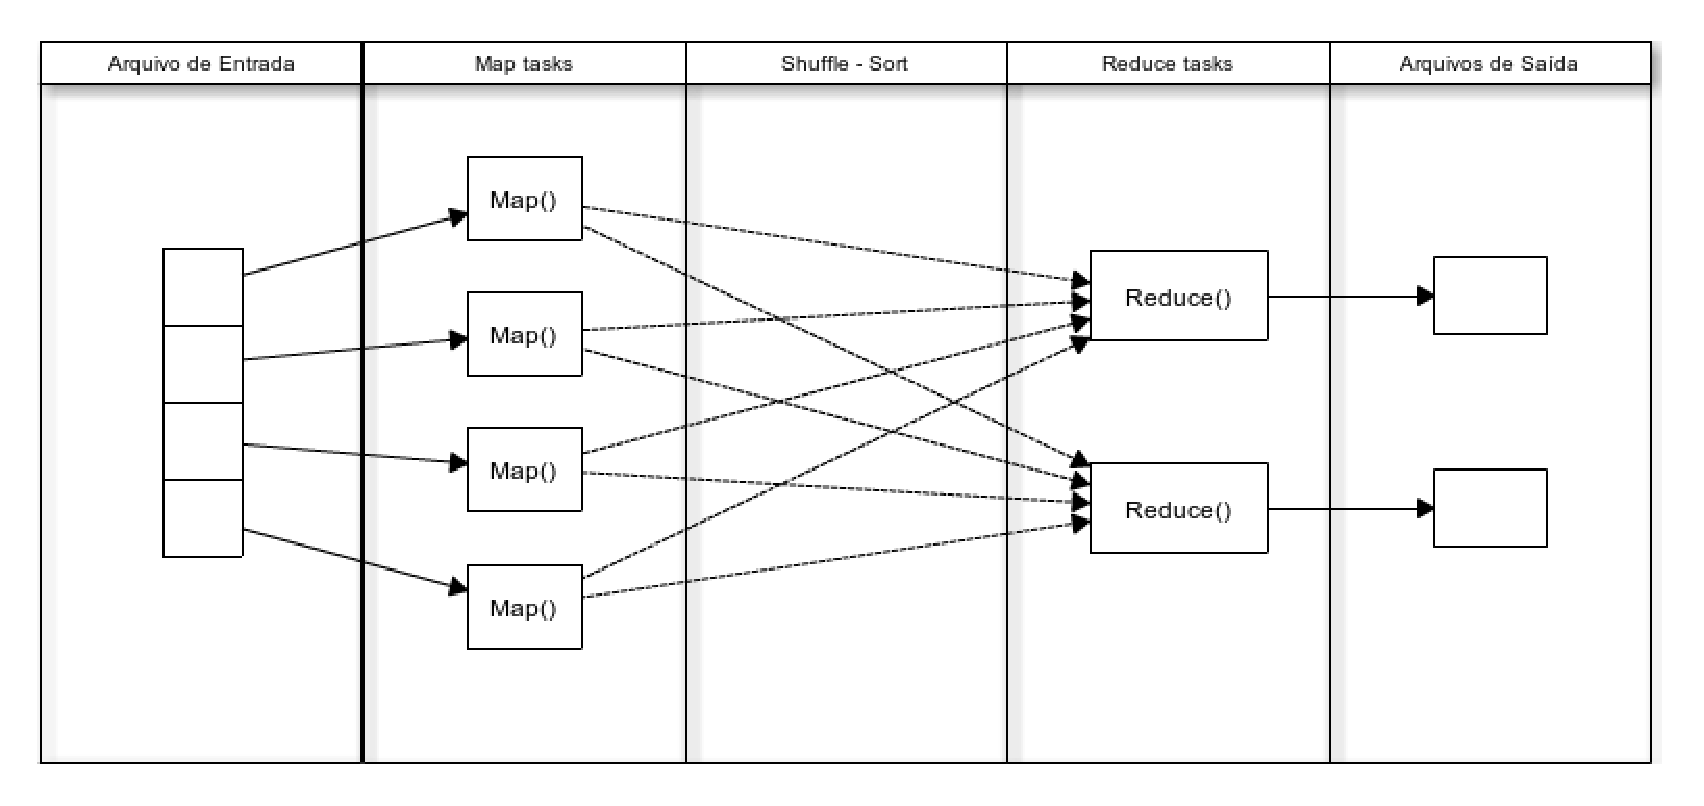
\includegraphics[keepaspectratio=true,scale=0.5]
	  {figuras/mapreduce.eps}
	\caption[Fluxo de um programa MapReduce]{Fluxo de um programa MapReduce
	\protect\linebreak Fonte: Autor}
	\label{fig-mapreduce}
\end{figure}
\FloatBarrier

Nas fases \textit{shuffle} e \textit{sort} os pares intermediários são agrupados e ordenados de acordo com sua chave. Este processo é realizado pelo \textit{framework} e será detalhado nas seções seguintes, sendo uma das etapas mais complexas de todo fluxo. Por fim, as \textit{reduce tasks} recebem como entrada os valores resultantes das etapas \textit{shuffle} e \textit{sort}. Para cada entrada \textit{\{chave, lista(valores)\}} existente, uma \textit{reduce task} executa uma chamada a função \textit{reduce} especificada pelo desenvolvedor.

\subsection{Contador de Palavras}
\label{sec-wc}

Um exemplo simples da aplicabilidade do MapReduce pode ser observado em um problema definido como contador de palavras. Suponha que exista um arquivo de texto com várias palavras inseridas, onde o objetivo seja contar a quantidade de ocorrências de cada uma destas palavras ao longo de todo texto. A princípio parece ser uma atividade trivial, entretanto se o tamanho do arquivo estiver na ordem de gigabytes e aumentarmos a quantidade de arquivos a serem processados o tempo de execução aumentará consideravelmente, tornando-se inviável realizar esta análise.

Uma alternativa para contornar este problema seria o uso da programação paralela, analisando os arquivos em diferentes processos, utilizando quantas \textit{threads} fossem necessárias. Todavia esta solução não é a mais eficiente, já que os arquivos podem apresentar diferentes tamanhos, ou seja, alguns processos seriam finalizados em um intervalo de tempo menor, impossibilitando maximizar a capacidade de processamento. 

Uma abordagem mais eficiente seria separar todos os arquivos em blocos pré definidos e então dividi-los em processos distintos. Esta solução requer um mecanismo de sincronização complexo e de difícil implementação. Seria necessário agrupar todas as palavras e suas respectivas ocorrências em cada uma das \textit{threads} nos diferentes processos em execução. E mesmo assim a capacidade de processamento estaria limitada a apenas uma máquina.

Este problema que se mostrou complexo possui uma solução simples e de fácil construção quando utiliza-se a abordagem apresentada pelo paradigma MapReduce. Nesta situação torna-se necessária apenas a definição de uma função \textit{map} para realizar a contagem de cada palavra presente nos arquivos de entrada, e também de uma função \textit{reduce} para agrupar cada uma destas palavras e realizar a contagem final dos registros de ocorrências. Um pseudo código com as funções \textit{map} e \textit{reduce} para este problema são apresentadas no código \ref{cod-mapreduce-google}.

\lstinputlisting[float,
		frame=single,
		label=cod-mapreduce-google,
		style=abnt,
		caption={[Pseudo código MapReduce]Pseudo código MapReduce
		\protect\linebreak Fonte: \cite{ghemawatMapreduce2008}}]
		{codigos/mapreduce-pseudo}
\FloatBarrier

No código \ref{cod-mapreduce-google} o programa MapReduce divide todos os arquivos de entrada em \textit{input splits}, na qual a chave do par \textit{\{chave, valor\}} é composta pelo número do respectivo \textit{input split}, enquanto o valor é o próprio conteúdo de sua parte no texto. Para cada par de entrada uma função \textit{map} será chamada e realizará quebra da linha em palavras. Cada um destes \textit{tokens} é associado ao valor 1, gerando pares de saída no formato \textit{\{palavra, 1\}}.

O \textit{framework} MapReduce realiza as etapas \textit{shuffle} e \textit{sort} para agrupar e ordenar os resultados das \textit{map tasks}. Em seguida para cada chave existente será realizada uma chamada a uma função \textit{reduce}, na qual é responsável por percorrer uma lista efetuando a soma dos valores encontrados. O resultado obtido é registrado em um arquivo de saída. A figura \ref{fig-mapreduce-word-count} apresenta o fluxo completo da execução de um programa MapReduce para o problema da contagem de palavras.

\begin{figure}[ht!]
	\centering
	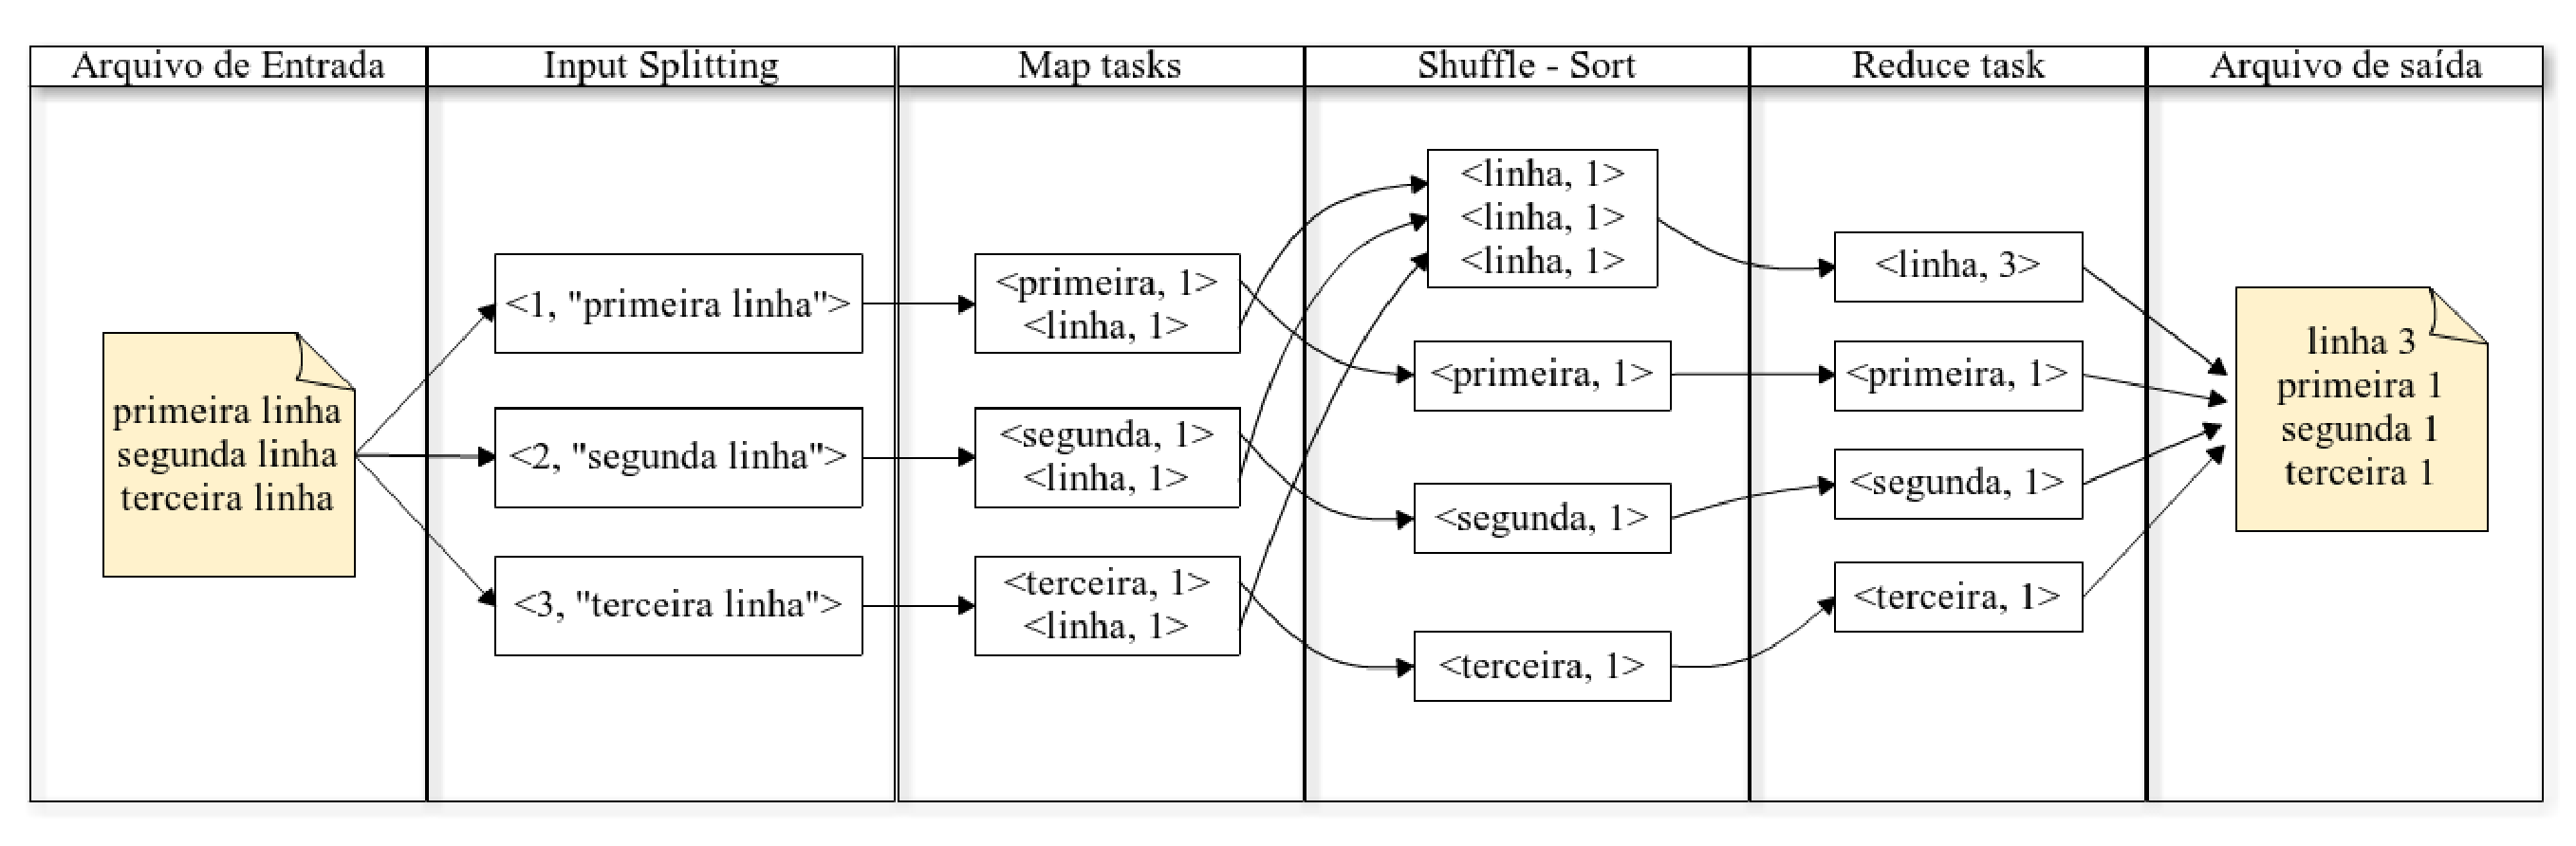
\includegraphics[keepaspectratio=true,scale=0.36]
	  {figuras/mapreduce-word-count.eps}
	\caption[Fluxo de atividades para o contador de palavras]{Fluxo de atividades para o contador de palavras
	\protect\linebreak Fonte: Autor}
	\label{fig-mapreduce-word-count}
\end{figure}
\FloatBarrier

\subsection{Arquitetura}

O modelo MapReduce foi criado pela Google para que os programas escritos neste estilo funcional fossem automaticamente paralelizados e executados em um \textit{cluster} composto por hardwares de baixo custo \cite{ghemawatMapreduce2008}. As responsabilidades do \textit{framework} consistem em particionar as entradas em \textit{input splits}, gerenciar a execução e comunicação entre os processos do programa ao longo das máquinas e também tratar as falhas que podem ocorrer em cada nó da rede. De acordo com \citeonline{ghemawatMapreduce2008}, com este cenário um desenvolvedor sem nenhuma experiência em computação paralela seria capaz de desenvolver soluções aplicadas para este contexto. 

Este modelo pode ser aplicado em diversas plataformas, mas o foi projetado principalmente para ser executado sobre o sistema de arquivos distribuídos GFS. Na figura \ref{fig-mapreduce-google} é apresentada a arquitetura do MapReduce proposta pela Google, através dela é possível visualizar que um \textit{cluster} é composto por dois tipos de nós: um \textit{master} e diversos \textit{workers}.

Inicialmente os arquivos de entrada são divididos em \textit{input splits} de aproximadamente 64MB, assim como o tamanho dos blocos de arquivos no GFS e também no HDFS. Segundo \citeonline{ghemawatMapreduce2008}, as \textit{map tasks} criadas para cada uma destas entradas são espalhadas pelo \textit{cluster} e executadas em paralelo nos nós do tipo \textit{worker}. As \textit{reduce tasks} criadas para computar os valores intermediários também são processadas em \textit{workers}.

\begin{figure}[ht!]
	\centering
	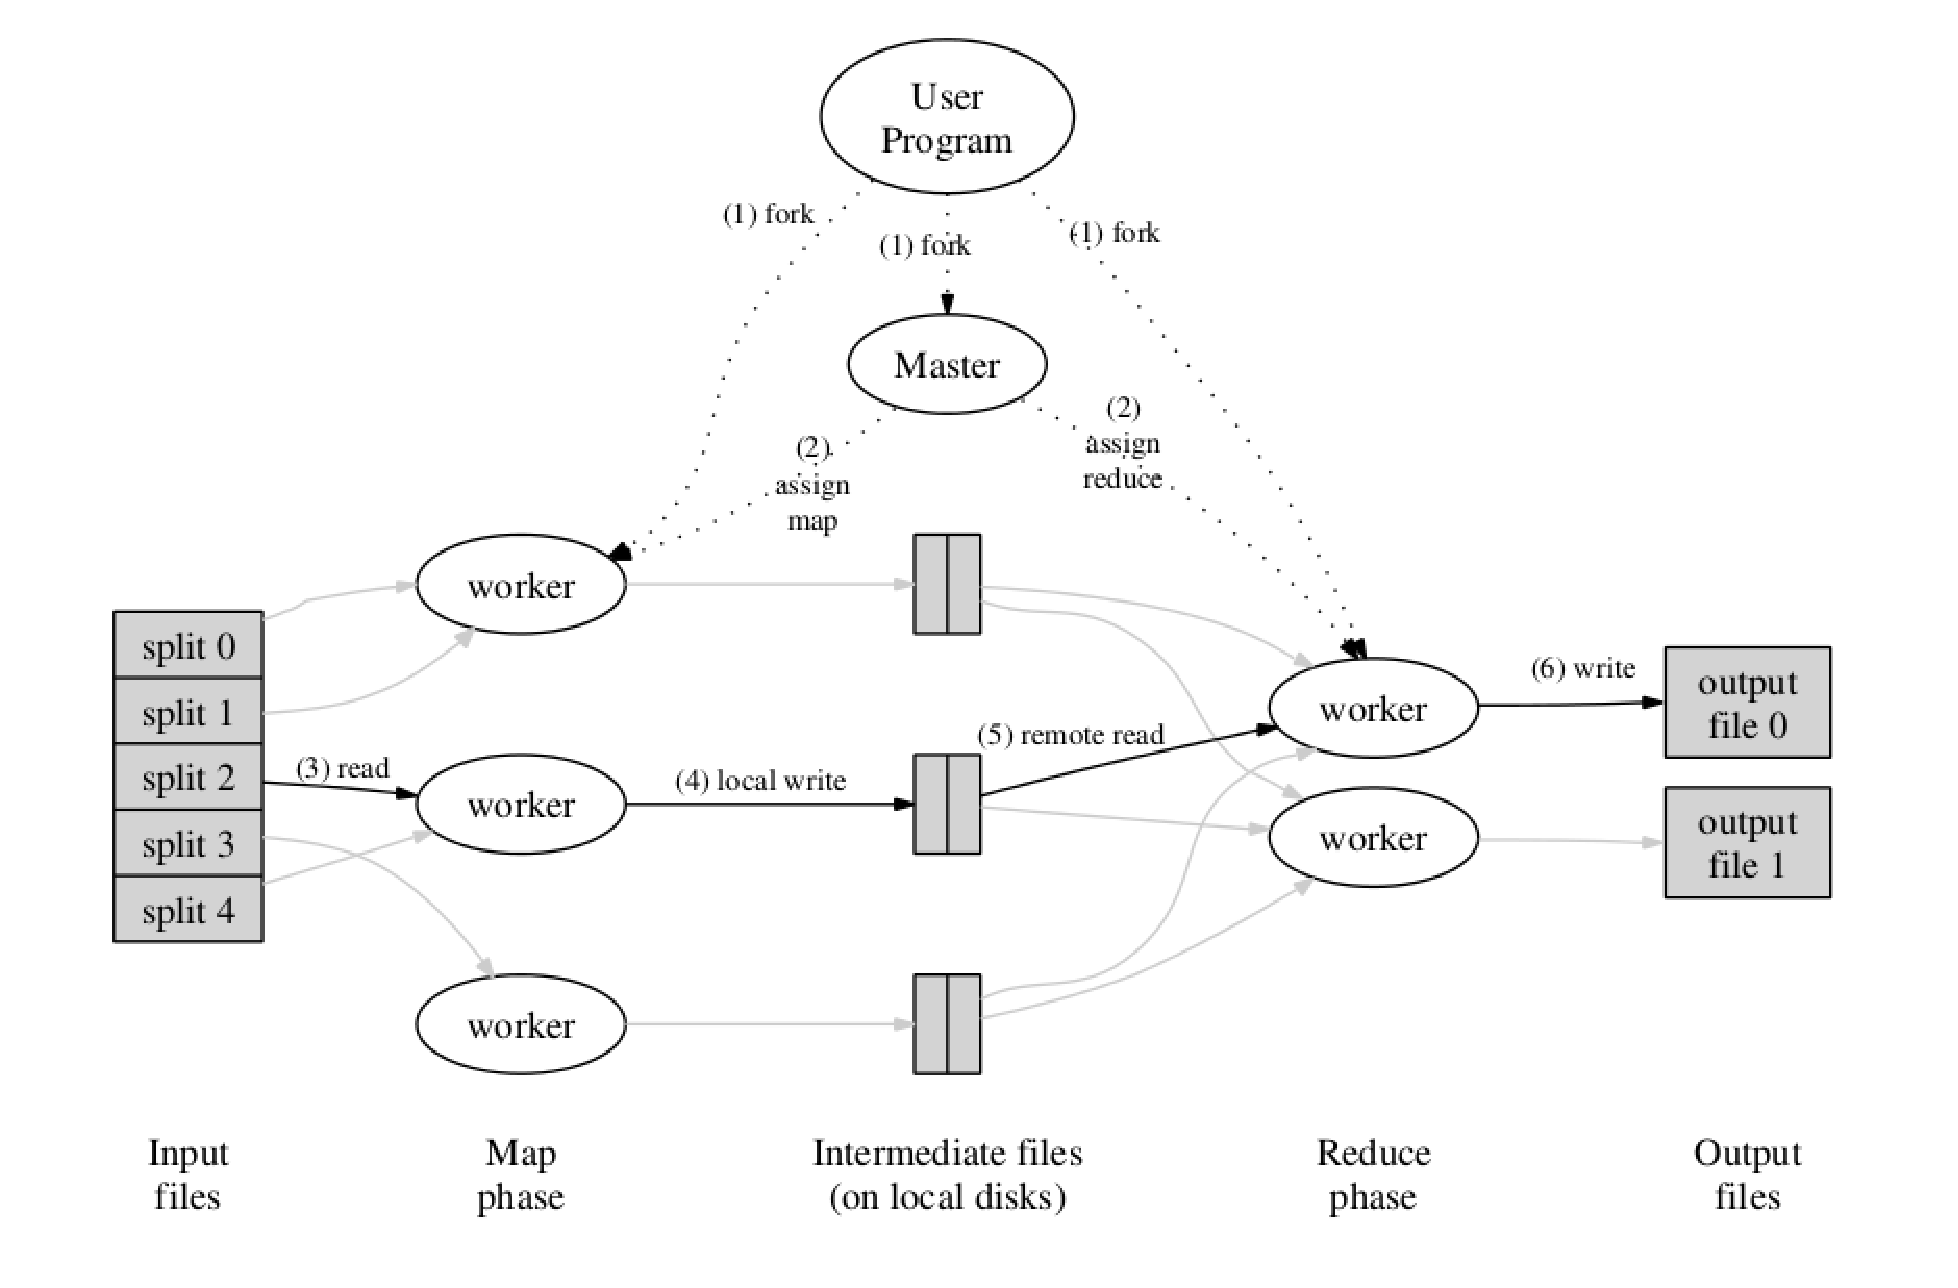
\includegraphics[keepaspectratio=true,scale=0.5]
	  {figuras/mapreduce-google.eps}
	\caption[Arquitetura MapReduce]{Arquitetura MapReduce
	\protect\linebreak Fonte: \cite{ghemawatMapreduce2008}}
	\label{fig-mapreduce-google}
\end{figure}
\FloatBarrier

O \textit{MapReduce job} submetido pelo usuário faz o cálculo de quantas \textit{map tasks} serão necessárias para realizar o processamento dos \textit{input splits}. O nó \textit{master} então possui a tarefa de distribuir as \textit{map tasks} e também as \textit{reduce tasks} para os \textit{workers} disponíveis na rede. De acordo com \citeonline{ghemawatMapreduce2008}, o nó \textit{master} também é responsável por manter o estado de todas as funções \textit{map} e \textit{reduce} que são executadas no \textit{cluster}. Estes dados informam se uma determinada tarefa está inativa, em progresso ou finalizada. 

A máquina \textit{master} também monitora os \textit{workers} através de \textit{pings} que são realizados periodicamente. Caso um \textit{worker} não responda será declarado como indisponível, todas as tarefas deste nó serão reagendadas para serem executadas por outro \textit{worker}. Esta preocupação em monitorar os nós ao longo do \textit{cluster} ocorre porque segundo \citeonline{ghemawatMapreduce2008}, o MapReduce é uma biblioteca projetada para auxiliar no processamento de dados em larga escala ao longo de milhares de máquinas, portanto precisa prover um mecanismo eficiente para tolerar as falhas que ocorrem em computadores da rede.

A largura de banda da rede pode ser considerada um recurso crítico mediante ao contexto apresentado até o momento, a utilização da rede para transportar dados deve ser otimizada ao máximo para que este fator não prejudique o desempenho de um programa MapReduce. Em virtude disso o MapReduce procura tirar vantagem do fato de que os arquivos de entrada são persistidos no disco local dos \textit{workers}. Portanto o \textit{master} obtém a localização de cada \textit{input split} e procura executar as \textit{map tasks} exatamente nestas máquinas \cite{ghemawatMapreduce2008}. Desta forma a execução da fase de mapeamento é realizada localmente, sem consumir os recursos da rede. Segundo \citeonline{white2012}, este processo pode ser definido como \textit{data locality optimization}.

Por sua vez, as \textit{reduce tasks} não possuem a vantagem de serem executadas localmente, pois sua entrada pode estar relacionada às saídas de um conjunto de diferentes \textit{map tasks}. Portanto os valores intermediários gerados pelas funções \textit{map} devem ser transportados pela rede até a máquina onde a função \textit{reduce} está sendo processada.

O Hadoop MapReduce apresenta uma implementação \textit{open-source} consolidada para o modelo MapReduce, na qual é construída a partir da linguagem de programação Java \cite{hadoopSiteMapReduce}, diferentemente do \textit{framework} original desenvolvido em C++ pela Google. A arquitetura do MapReduce pode ser facilmente associada ao paradigma mestre/escravo. A máquina \textit{master} representa o mestre do sistema, enquanto os \textit{workers} simbolizam os escravos. No contexto proposto pelo Hadoop estes elementos são identificados como \textit{jobtracker} e os \textit{tasktrackers}, respectivamente. A figura \ref{fig-mapreduce-arquitetura} ilustra a arquitetura do Hadoop MapReduce.

\begin{figure}[ht!]
	\centering
	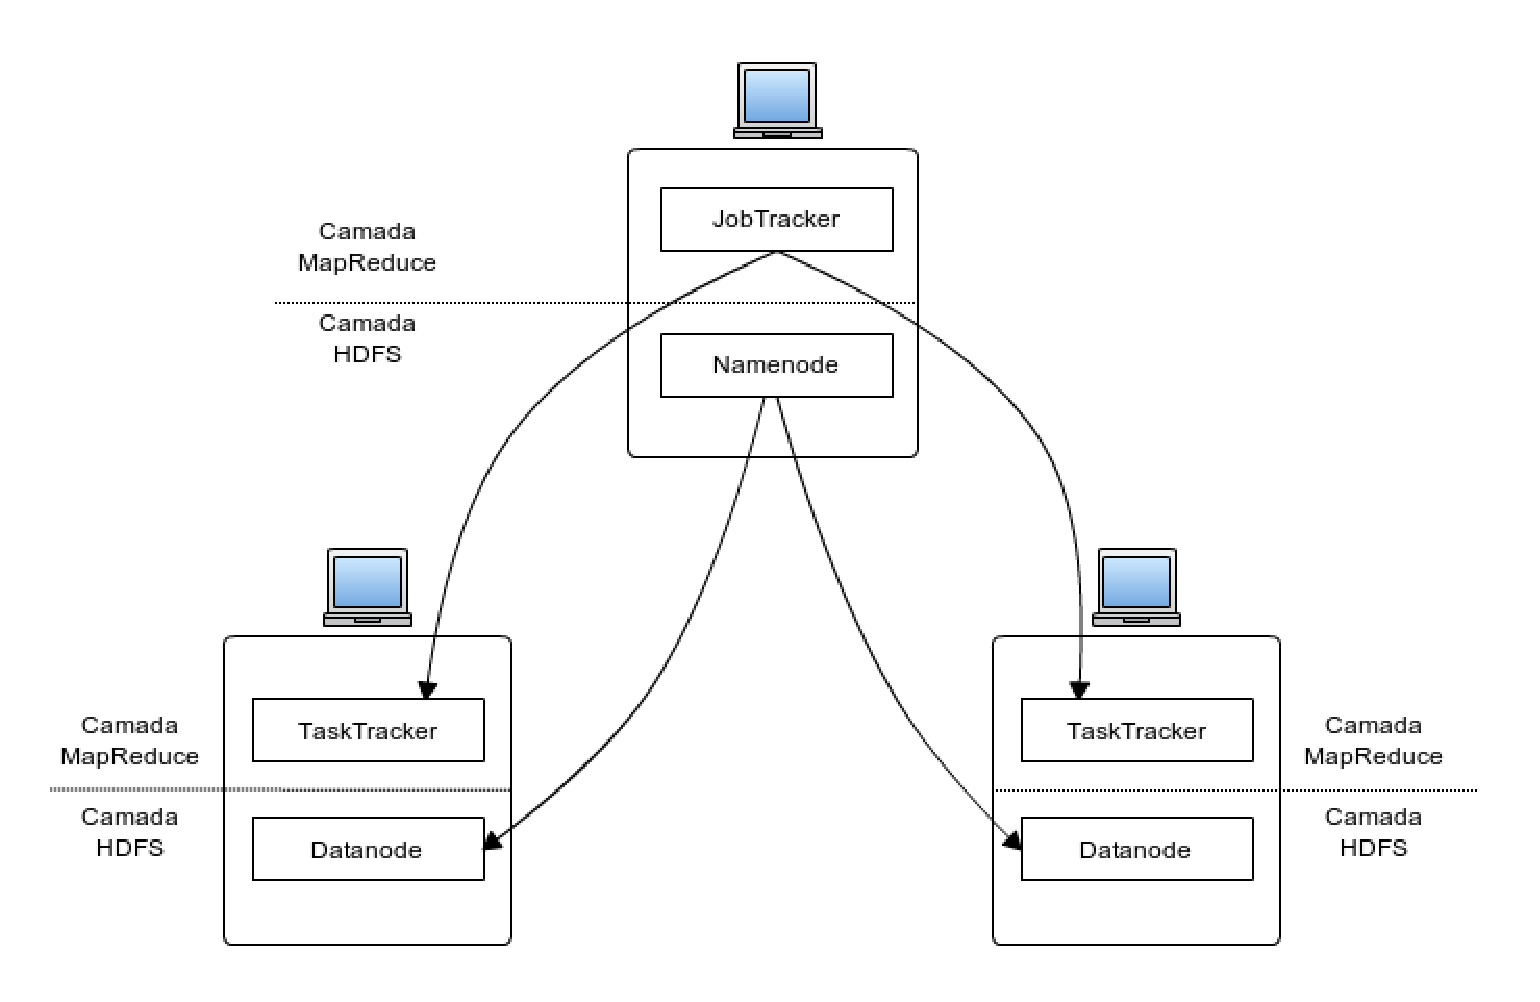
\includegraphics[keepaspectratio=true,scale=0.6]
	  {figuras/mapreduce-arquitetura.eps}
	\caption[Arquitetura de um cluster Hadoop]{Arquitetura de um cluster Hadoop
	\protect\linebreak Fonte: Autor}
	\label{fig-mapreduce-arquitetura}
\end{figure}
\FloatBarrier

Assim como no ambiente proposto pela Google, o Hadoop MapReduce também é executado sobre um sistema de arquivos distribuídos em larga escala, no caso o HDFS. Segundo \citeonline{venner2009}, é comum o \textit{jobtracker} e o \textit{namenode} estarem localizados na mesma máquina do \textit{cluster}, especialmente em instalações reduzidas.

\subsection{\textit{Shuffle e Sort}}

Uma das responsabilidades do \textit{framework} MapReduce é garantir que os pares intermediários \textit{\{chave, valor\}} resultantes das funções \textit{maps} sejam ordenados, agrupados e passados como parâmetro para as funções de redução. Esta fase é classificada como \textit{shuffle} e \textit{sort}. De acordo com \citeonline{white2012} esta é a área do código base do Hadoop que está em contínua evolução, podendo ser classificada como o núcleo do MapReduce. A figura \ref{fig-shuffle} ilustra os processos de \textit{shuffle} e \textit{sort} que ocorrem entre a execução das funções \textit{map} e \textit{reduce}.

\begin{figure}[ht!]
	\centering
	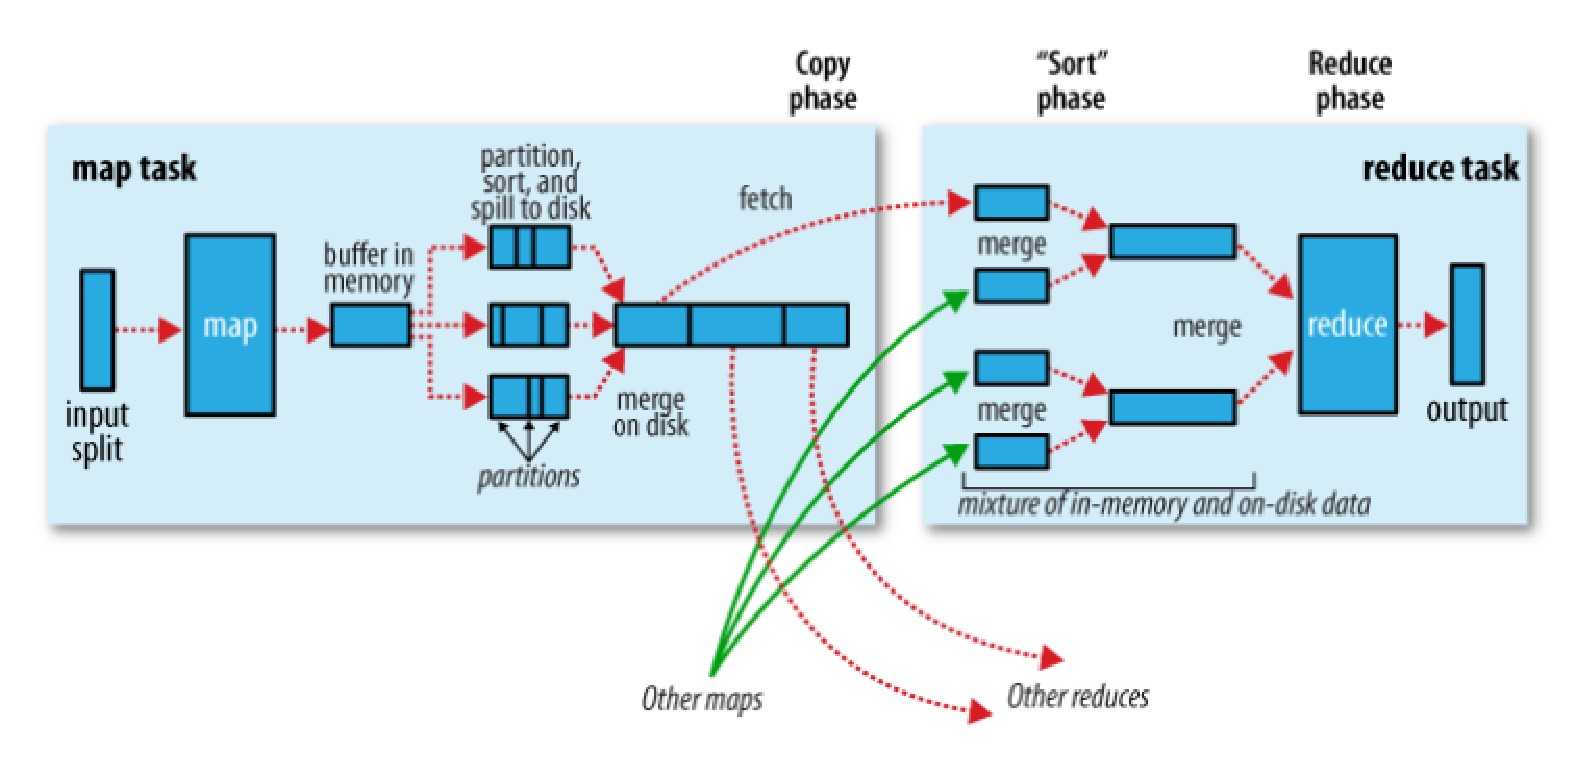
\includegraphics[keepaspectratio=true,scale=0.6]
	  {figuras/shuffle.eps}
	\caption[Fluxograma das etapas Shuffle e Sort]{Fluxograma das etapas Shuffle e Sort
	\protect\linebreak Fonte: \cite{white2012}}
	\label{fig-shuffle}
\end{figure}
\FloatBarrier

Durante a execução de uma função \textit{map} os pares \textit{\{chave, valor\}} resultantes são escritos em um \textit{buffer} na memória na medida em que são gerados. Os registros são divididos em R partições, na qual R representa a quantidade de funções \textit{reduce} que seriam necessárias para processar os resultados. Em seguida as partições são ordenadas de acordo com as chaves e escritas no disco local. Segundo \citeonline{white2012}, Os resultados das \textit{map tasks} são escritos no próprio disco da máquina porque se tratam de arquivos intermediários, não há necessidade de armazená-los no sistema de arquivos distribuídos. Esta etapa de particionamento e ordenação é denominada \textit{shuffle}.

Após o término de uma \textit{map task} ocorre a fase de cópia. Nesta etapa as máquinas onde serão executadas as \textit{reduce tasks} são informadas pelo \textit{master} sobre a localização das partições a elas destinadas. As partições geradas pelas \textit{map tasks} são ordenadas localmente justamente para auxiliar neste procedimento. Ao término da cópia de todas as partições ocorre a fase \textit{sort}, onde os resultados são agrupados por chave, mantendo-se a ordenação pela mesma. Desta forma as entradas para as funções de redução estão prontas para serem computadas.

